\section{Awareness}
\label{chp: awareness}

Et sykehus er en organisasjon med mange informasjonskilder, stress, variasjon mellom rutinearbeid og uforutsette aktiviteter, og ansatte som stadig er på forskjellige steder. Kommunikasjon og oversikt er derfor svært viktig for å sikre god pasientomsorg og sikkerhet \cite{Klemets12}.

\subsubsection{Awareness}
Awareness er et svært uklart og komplekst begrep med mange definisjoner og konseptualiseringer \cite{KlemetsRedundancy, Gutwin04, Schmidt02}. Begrepet brukes i utallige sammenhenger, og mange forskere blir stadig mindre komfortable med å bruke begrepet i seg selv. For å komme til en slags konseptuell klarhet i hva awareness betyr må vi innse at det ikke gir mening å se på awareness som noe i seg selv, men som noe som refererer til awareness \emph{om} noe \cite{Schmidt02}. Dermed oppstår konsepter som blant annet sosial, eller kontekstformidlet sosial awareness \cite{Bardram04}, generell awareness \cite{Gross13}, romlig og tidsmessig awareness \cite{Randell}, gruppe-awareness \cite{Gutwin04}, perifer-, bakgrunns-, passiv- og gjensidig awareness \cite{Schmidt02}. Dette gir også mange, og til dels ulike definisjoner. Dourish og Bellotti (1992)\nocite{Dourish92} definerer awareness som \emph{"an understanding of the activities of others, which provides a context for your own activity"}. En definisjon av situasjonell awareness finner vi i \cite{Endsly95}, \emph{"oppfattelsen av elementene i omgivelsene avgrenset av tid og rom, forståelsen av deres mening, og prognosen for deres status i nær fremtid"}. I \cite{Gross13} er generell awareness definert som \emph{"den gjennomgripende opplevelsen av å vite hvem som befinner seg i nærheten, hva de driver med, om de er relativt opptatt eller kan engasjeres"}. Bardrams (2004) konsept kontekstformidlet sosial awareness har som mål å minimere uønskede forstyrrelser mellom mobile kolleger ved å øke deres sosiale awareness ved hjelp av kontekstbevisste systemer. Bardram et al. (2006) trekker frem tre av disse som spesielt viktige i helseomsorgen etter å ha gjort observasjoner på koordinasjon i et sykehusmiljø: (1) Sosial awareness, som hvor kolleger befinner seg og deres aktiviteter, (2) romlig awareness, hva foregår på en gitt lokasjon og (3) tidsmessig awareness, som omhandler tidligere, nåværende og fremtidige aktiviteter.

\noindent
I Cabitza et al. (2005) \nocite{Cabitza} finner vi at awareness også kan oppstå som et resultat av redundans, og skiller mellom tre typer: (1) redundans av funksjon, (2) redundans av innsats og (3) redundans av data. Redundans av funksjon innebærer at flere individer har overlappende funksjoner eller ferdigheter, slik at flere kan utføre samme oppgave. Redundans av innsats oppstår når utførte oppgaver gjøres på nytt, eller man bruker flere ressurser enn nødvendig for å løse en oppgave. Et typisk eksempel på dette er menneskelig kommunikasjon, hvor man gjentar en beskjed for å sørge for at den oppfattes eller for å vise at den er forstått. Redundans av data innebærer at lik eller lignende informasjon finnes på flere steder, for eksempel både digitalt og på papir, eller på flere digitale enheter. Teknologi kan bidra effektiv spredning informasjon, for eksempel gjennom å tilby data på personlige enheter som mobiltelefoner, samt på delte offentlige enheter som tavler og skjermer. Dette fører til økt redundans av data, men mindre redundans av innsats og dermed mer effektiv koordinasjon av arbeid.

\noindent
Dersom en ser bort fra alle konseptualiseringer og definisjoner kan man som i Randell (2010) dele awareness i to kategorier: (1) Biprodukt-awareness, hvor awareness oppnås gjennom aktivitetene i seg selv, uten at det krever merarbeid for individene. Og (2) awareness ved merarbeid, hvor individene må gjøre ekstra arbeid for å opprettholde awareness. 

\noindent
Selv om god pasientomsorg er avhengig av sykepleierenes oversikt over situasjonen til enhver tid, må det også tas hensyn til pasienters og pårørendes privatliv. For å opprettholde en god balanse mellom disse, stilles det høye krav til sykepleierenes evne til å tilegne seg kunnskap om situasjonen på en måte som i minst mulig grad virker påtrengende for pasienter og pårørende, og at informasjon distribuert gjennom skjermer og tavler synlig for andre enn helsepersonell ikke krenker pasientenes privatliv \cite{Ebright10}.

\subsubsection{Awareness i CSCW}
Innen CSCW defineres awareness som det å "synliggjøre sine aktiviteter for, og oppfatte aktivitetene til, kolleger, for å støtte opp om samarbeidet dem i mellom". Awareness i denne sammenhengen ses på som essensiell for et godt samarbeid, og blir gjerne karakterisert som uanstrengt, eller biprodukt-awareness \cite{Randell}. 

\tikzstyle{mybox} = [draw=black, fill=white, very thick,
    rectangle, inner sep=10pt, inner ysep=20pt, rounded corners]
\tikzstyle{fancytitle} =[fill=black, text=white]
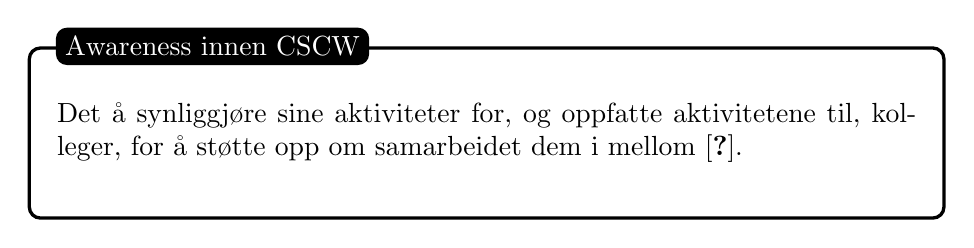
\begin{tikzpicture}
\node [mybox] (box){%
    \begin{minipage}{0.9\textwidth}
     Det å synliggjøre sine aktiviteter for, og oppfatte aktivitetene til, kolleger, for å støtte opp om samarbeidet dem i mellom \cite{Randell}.
    \end{minipage}
};
\node[fancytitle, rounded corners, right=10pt] at (box.north west) {Awareness innen CSCW};
\end{tikzpicture}%

\noindent
I følge både C. Heath et al. (2002) \nocite{Heath02} og Schmidt (2002), oppnås denne typen awareness gjennom kontinuerlig interaksjon med andre, og er på ingen måte en sinnstilstand eller passiv aktivitet. Dette underbygger tankene bak konseptualiseringen tilstandsawareness, hvor det kreves et visst nivå av kognitive ferdigheter for å til en hver tid kunne overvåke og oppdage endringer i omgivelsene. Dette skjer samtidig som man synliggjør for omgivelsene ens egen nåværende situasjon gjennom implisitte eller eksplisitte signaler. Med informasjonen man henter inn vil man da kunne danne seg et mentalt bilde av hvordan situasjonen til enhver tid er. I situasjoner hvor man ikke alltid er samlokalisert, som på et sykehus, kan bruk av kognitive gjenstander som tavler og skjermer være hensiktsmessig for å støtte opp under deling og innhenting av ovennevnte informasjon \cite{Bardram04}. 

\noindent
Erickson og Kellog (2000) argumenterer for at disse systemene bør være sosialt \emph{translucent} (på norsk: gjennomskinnelig) og skape "vinduer"\ og ikke barrierer mellom brukerne. Et slikt system har tre egenskaper: synlighet, awareness og ansvarlighet og støtter dermed samhandling ved å gjøre deltakerne og deres aktiviteter synlige for hverandre. Et eksempel som illustrerer slik transulence gis i \cite{Erickson00}: En dør som åpnes står i fare for å treffe en person som kommer fra motsatt side. Dersom døren er gjennomsiktig vil ikke en slik situasjon oppstå, da man vil \emph{se} at noen står på den andre siden av døren. Dette skaper awareness ved at \emph{jeg vet} at det står noen på den andre siden, og man vil dermed bli holdt ansvarlig for sin handling dersom man likevel skulle velge å åpne døren.

\noindent
Da vi i denne oppgaven ser på awareness blant sykepleiere og deres bruk av kognitive gjenstander for å støtte opp om dette, faller det seg naturlig å bruke definisjonen av awareness innen CSCW. Derfor, når vi i denne oppgaven bruker begrepet awareness, vil det være denne definisjonen vi sikter til.

